\documentclass[]{book}

\usepackage{import}
\usepackage{preamble}

\begin{document}

\noindent BECA / Huson / 11.2 Algebra II \hspace{2in} Name:\\*
19 October 2017
\begin{center}
{\Large Test: Linear functions and graphing}\\
\textit{Show your work. For graphs, use a pencil and straight edge.}
\end{center}

%\vspace{0.2 cm}


\subsection*{Solve equations}

Solve for the value of $x$.

\begin{enumerate}

\item   $2x-7=x$\\*[30pt]
\item   $12=x-5x$\\*[40pt]
\item   $\frac{1}{2}(5-x)=2x$\\*[60pt]
\item   $17=\frac{1}{2}x+4x-10$\\*[60pt]

\subsection*{Slope-intercept form}

What is the slope and $y$-intercept of each equation? 
\item   $y=3x-5$\\*[10pt]
\item   $6x+3y=9$\\*[40pt]


\subsection*{Point-slope form}

\item What is the equation of the line with a slope of 2 passing through the point $(2,1)$?\\*[20pt]
\item What is the equation of a line parallel to $y=-x+4$ through the point $(3, 2)$?\\*[20pt]
\item What is the slope of a line perpendicular to the line $2x-4y=5$?\\*[30pt]

\subsection*{Function substitution}
\item Given $f(x)=3x+17$. Simplify $f(1)$.\\*[20pt]
\item Given $\displaystyle f(x)=-\frac{(2+4x)}{3}$. Simplify $f(-1)$.\\*[20pt]

\subsection*{Interpreting graphs}
Answer each question with as an ordered pair, in the form $(x, y)$.
\item In the graph shown, what point has the greatest $y$ value?\\*[20pt]
\item Name three points with the same $y$ value.\\*[15pt]

\begin{figure}[!ht]
    \centering
    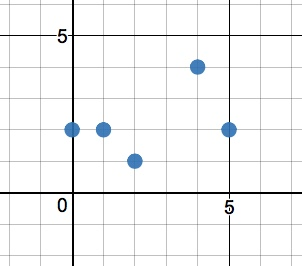
\includegraphics[width=0.35\textwidth]{discrete-domain-graph.jpeg}
\end{figure}

\newpage

\subsection*{Sketching a linear function}

\item   On the graph, sketch the lines and answer the question.
\begin{enumerate}
    \item Sketch line 1 given by $y=2x+4$.\\*[10pt]
    \item Sketch line 2 given by $x+2y=3$.\\*[20pt]
    \item Label the intersection of line 1 and line 2 as $P$.
    \item Are the two lines parallel, perpendicular, or neither?
\begin{figure}[!ht]
    \flushright
    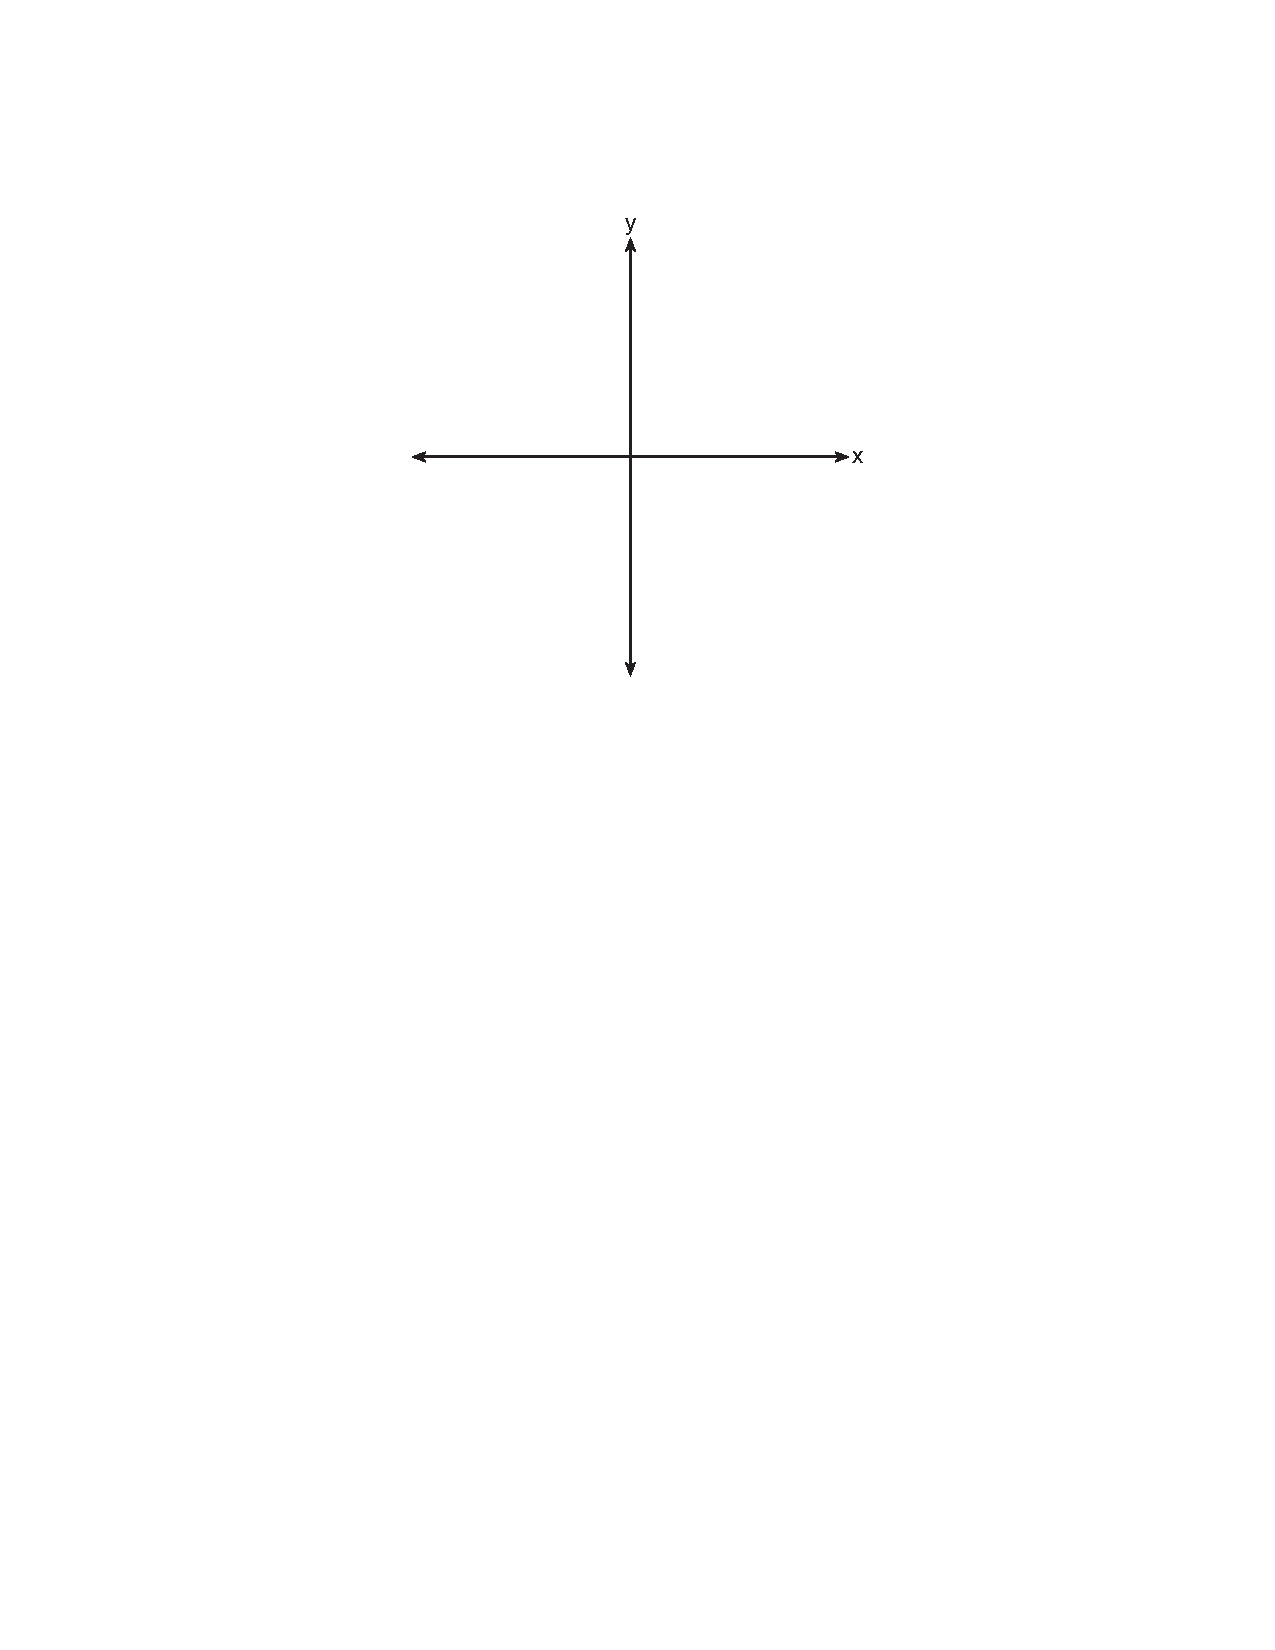
\includegraphics[width=0.6\textwidth]{simple-axes.pdf}
\end{figure}

\end{enumerate}


\newpage
\subsection*{Graphing linear functions}
Use pencil for graphs. Mark at least some of the values on each axis. Label each function with its name or equation. 
\item Graph the function $f(x)=\frac{1}{2}x+4$. 
\begin{enumerate}
    \item Write down the $y$-intercept.\\*[10pt]
    \item Write down the slope of $f(x)$.\\*[10pt]
    \item Label the intersection of $f(x)$ with the $x$-axis as the point $P$.
    \item Mark the point $Q (6, 2)$.
    \item A second line, $g(x)$, is parallel to $f(x)$ and passes through point $Q$. Plot $g(x)$ on the graph.
    \item What is the $y$-intercept of $g(x)$?\\*[10pt]
\end{enumerate}

\begin{figure}[!ht]
    \centering
    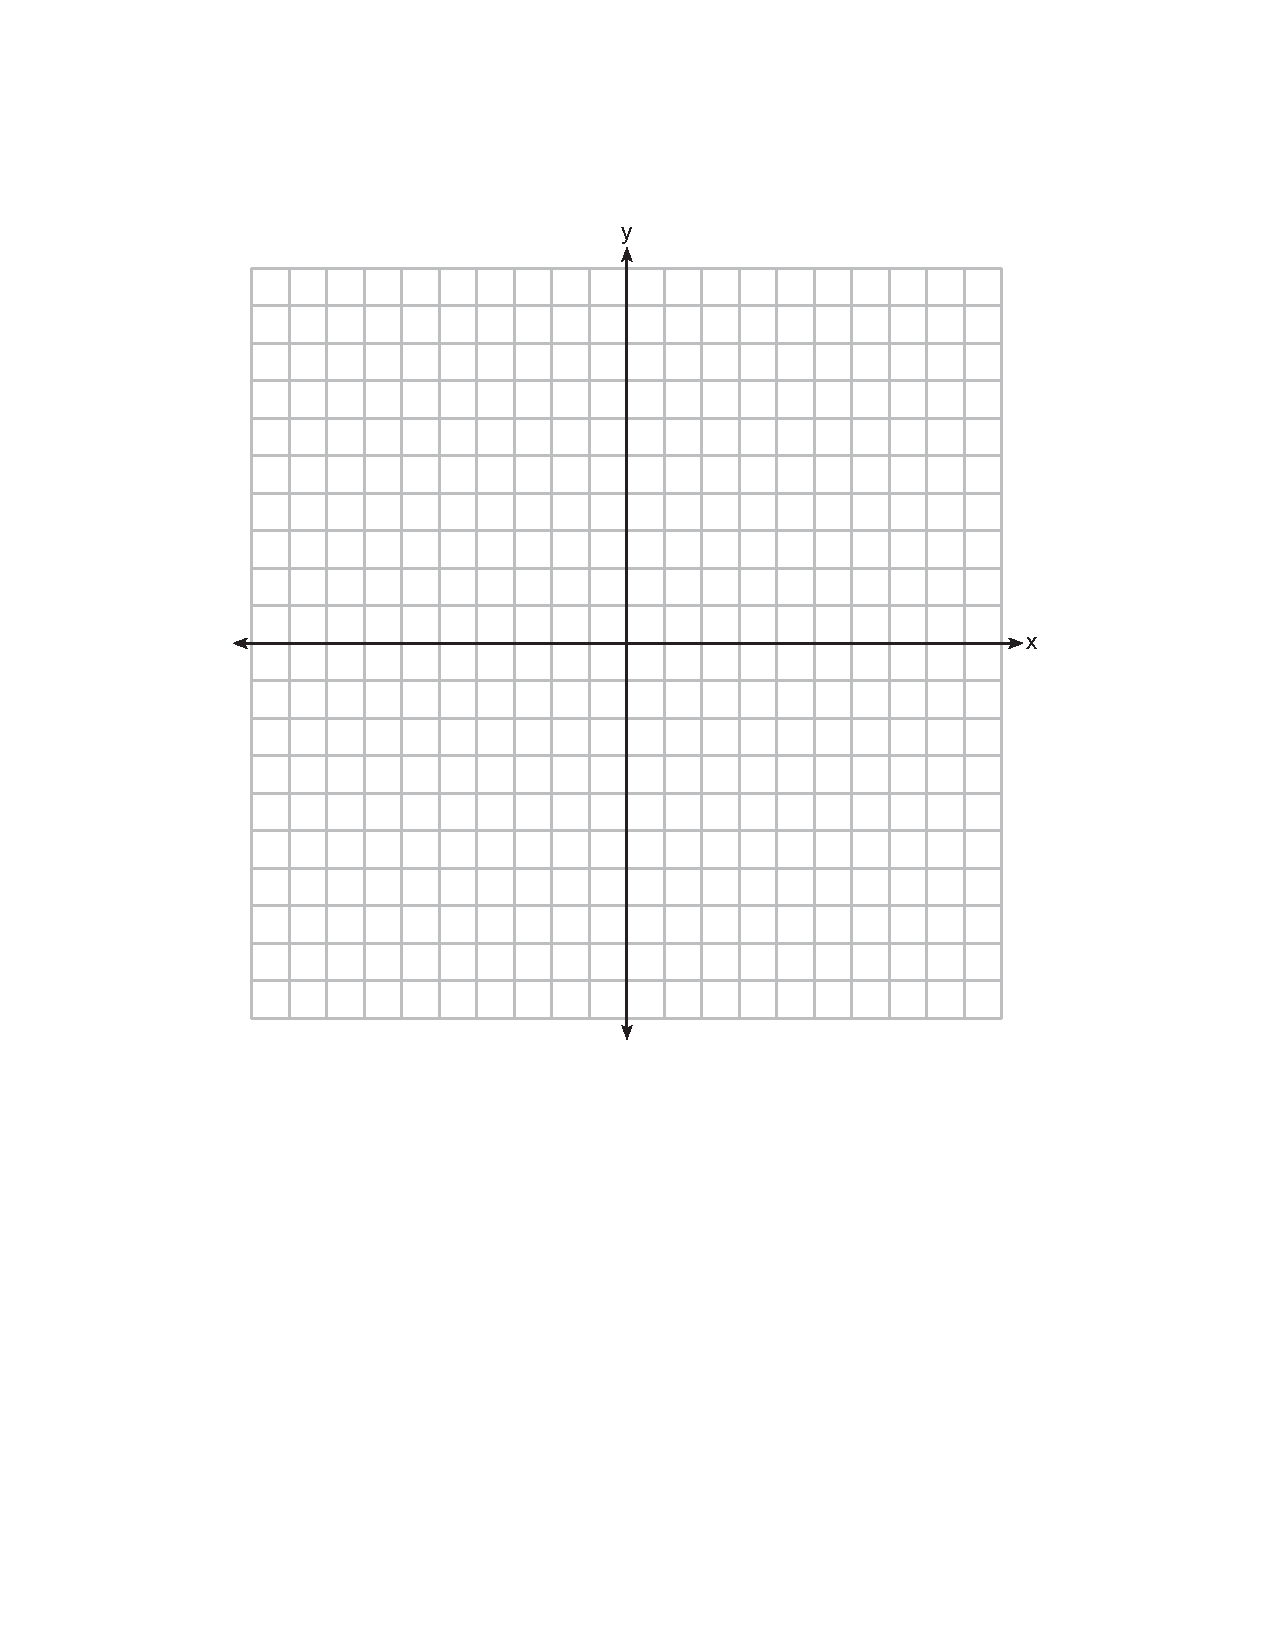
\includegraphics[width=0.75\textwidth]{regents-grid.pdf}
\end{figure}

\newpage
\item  
\begin{enumerate}
    \item Mark the point $P(3, -2)$ on the graph.
    \item The line $L_1$ has a $y$-intercept of 2 and passes through point $P$. Graph $L_1$.
    \item What is the slope of line $L_1$?\\*[20pt]
    \item What is the equation of line $L_1$?\\*[20pt]
    \item A second line, $L_2$ has the equation $x-y=-9$. Plot $L_2$ on the graph.
    \item What is the slope of $L_2$?\\*[30pt]
    \item Are the two lines $L_1$ and $L_2$ parallel, perpendicular, or neither?\\*[20pt]
    \item On the graph, mark the intersection of the two lines, the point $Q$, as an ordered pair.


\begin{figure}[!ht]
    \centering
    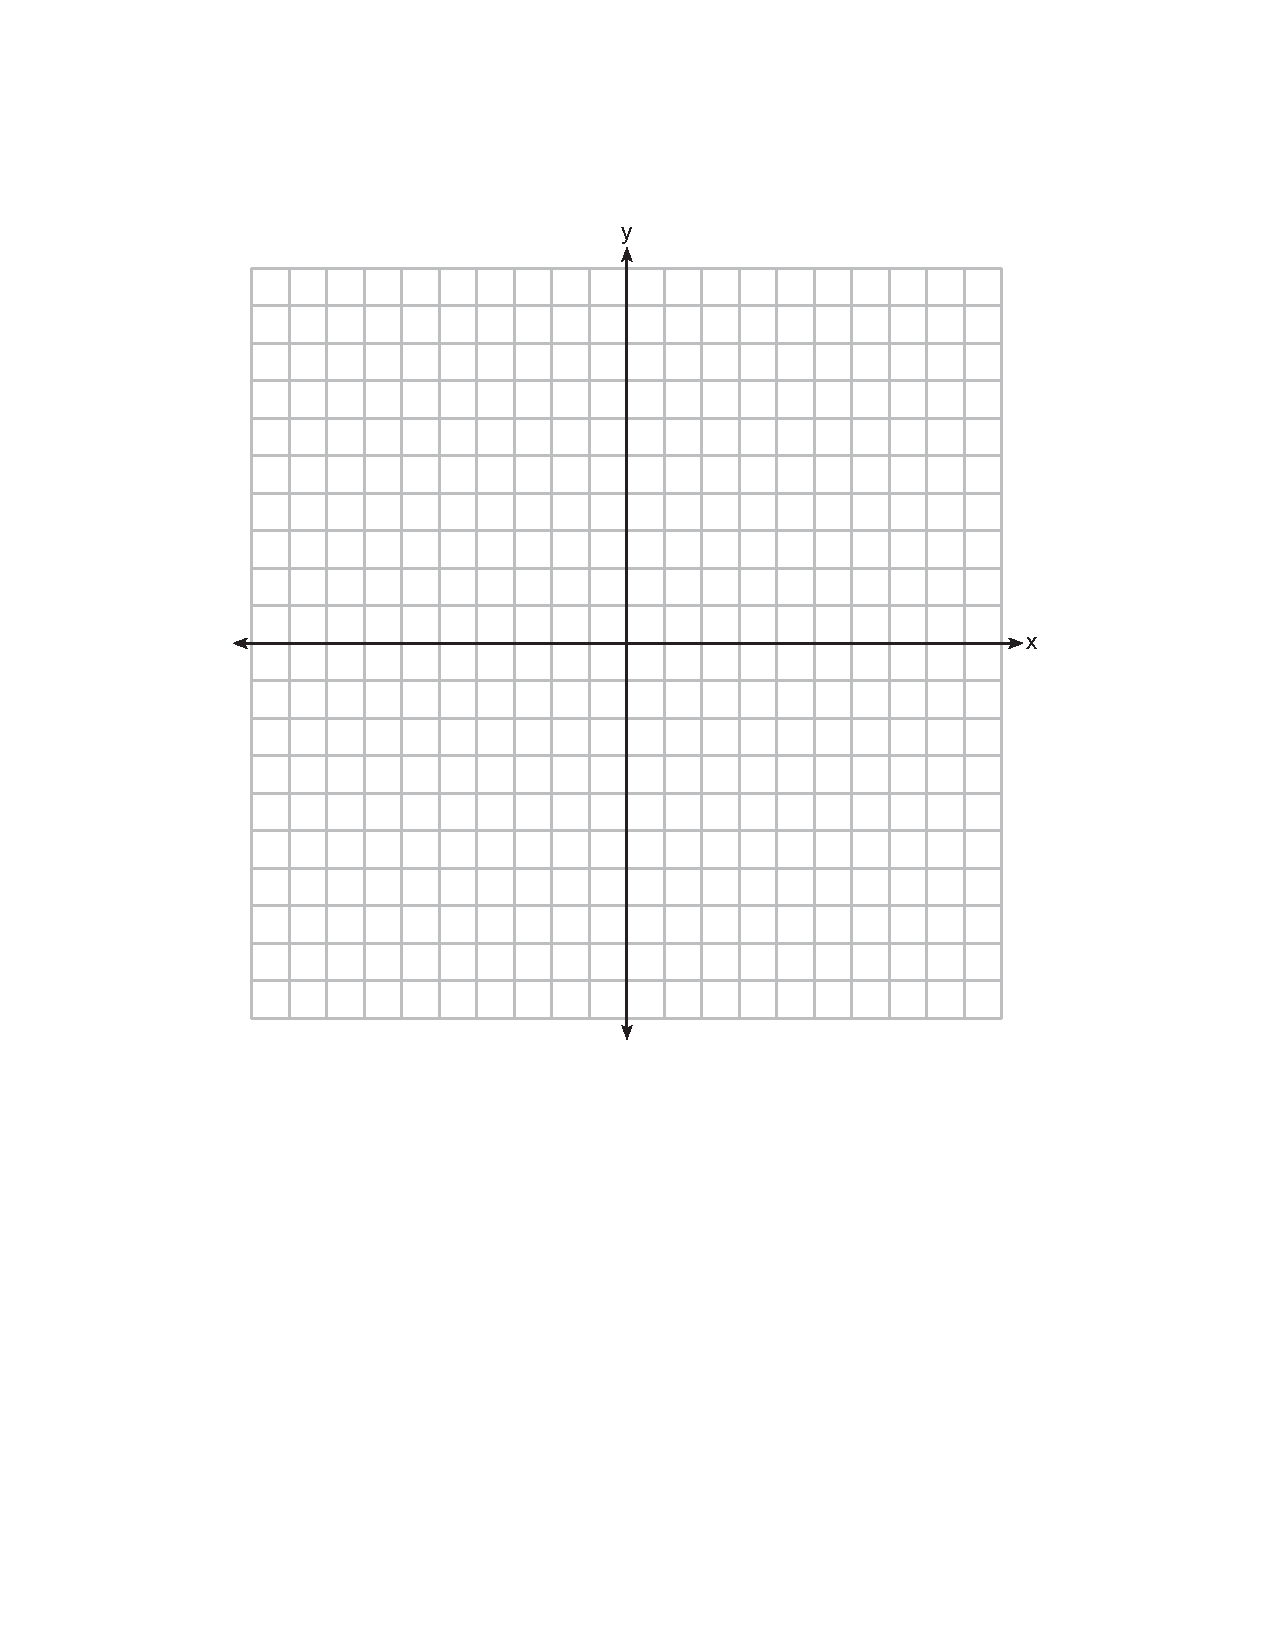
\includegraphics[width=0.65\textwidth]{regents-grid.pdf}
\end{figure}

    \item As a check, substitute the $x$ and $y$ values of $Q$ into $L_1$ and $L_2$ to show they satisfy each equation.

\end{enumerate}

\newpage
\subsection*{Model situations with linear functions}
Use pencil and a straight edge to make a scatter plot and line of best fit.
\item Label the axes as  $x$ and $y$. Mark at least some values (for example, 5, 10, 15, and 20). 
\begin{enumerate}
    \item Plot the values of $x$ and $y$ shown in the table.\\[5pt]
	\begin{tabular}{|l|c|c|c|c|c|c|c|c|c|}
	\hline
	$x$ & 1 & 3 & 7 & 8 & 11 & 12 & 15 & 17 & 19\\
	\hline
    $y$ & 8 & 8 & 11 & 13 & 13 & 12 & 10 & 16 & 17\\
	\hline
	\end{tabular}\\*[10pt]
	\item Draw a straight line of best fit that passes through the scatter plot of points, roughly representing their trend.
	\item Approximately what is the slope of the line of best fit?\\*[10pt]
	\item Approximately what is the $y$-intercept of the line of best fit?\\*[10pt]
\end{enumerate}

\begin{figure}[!ht]
    \centering
    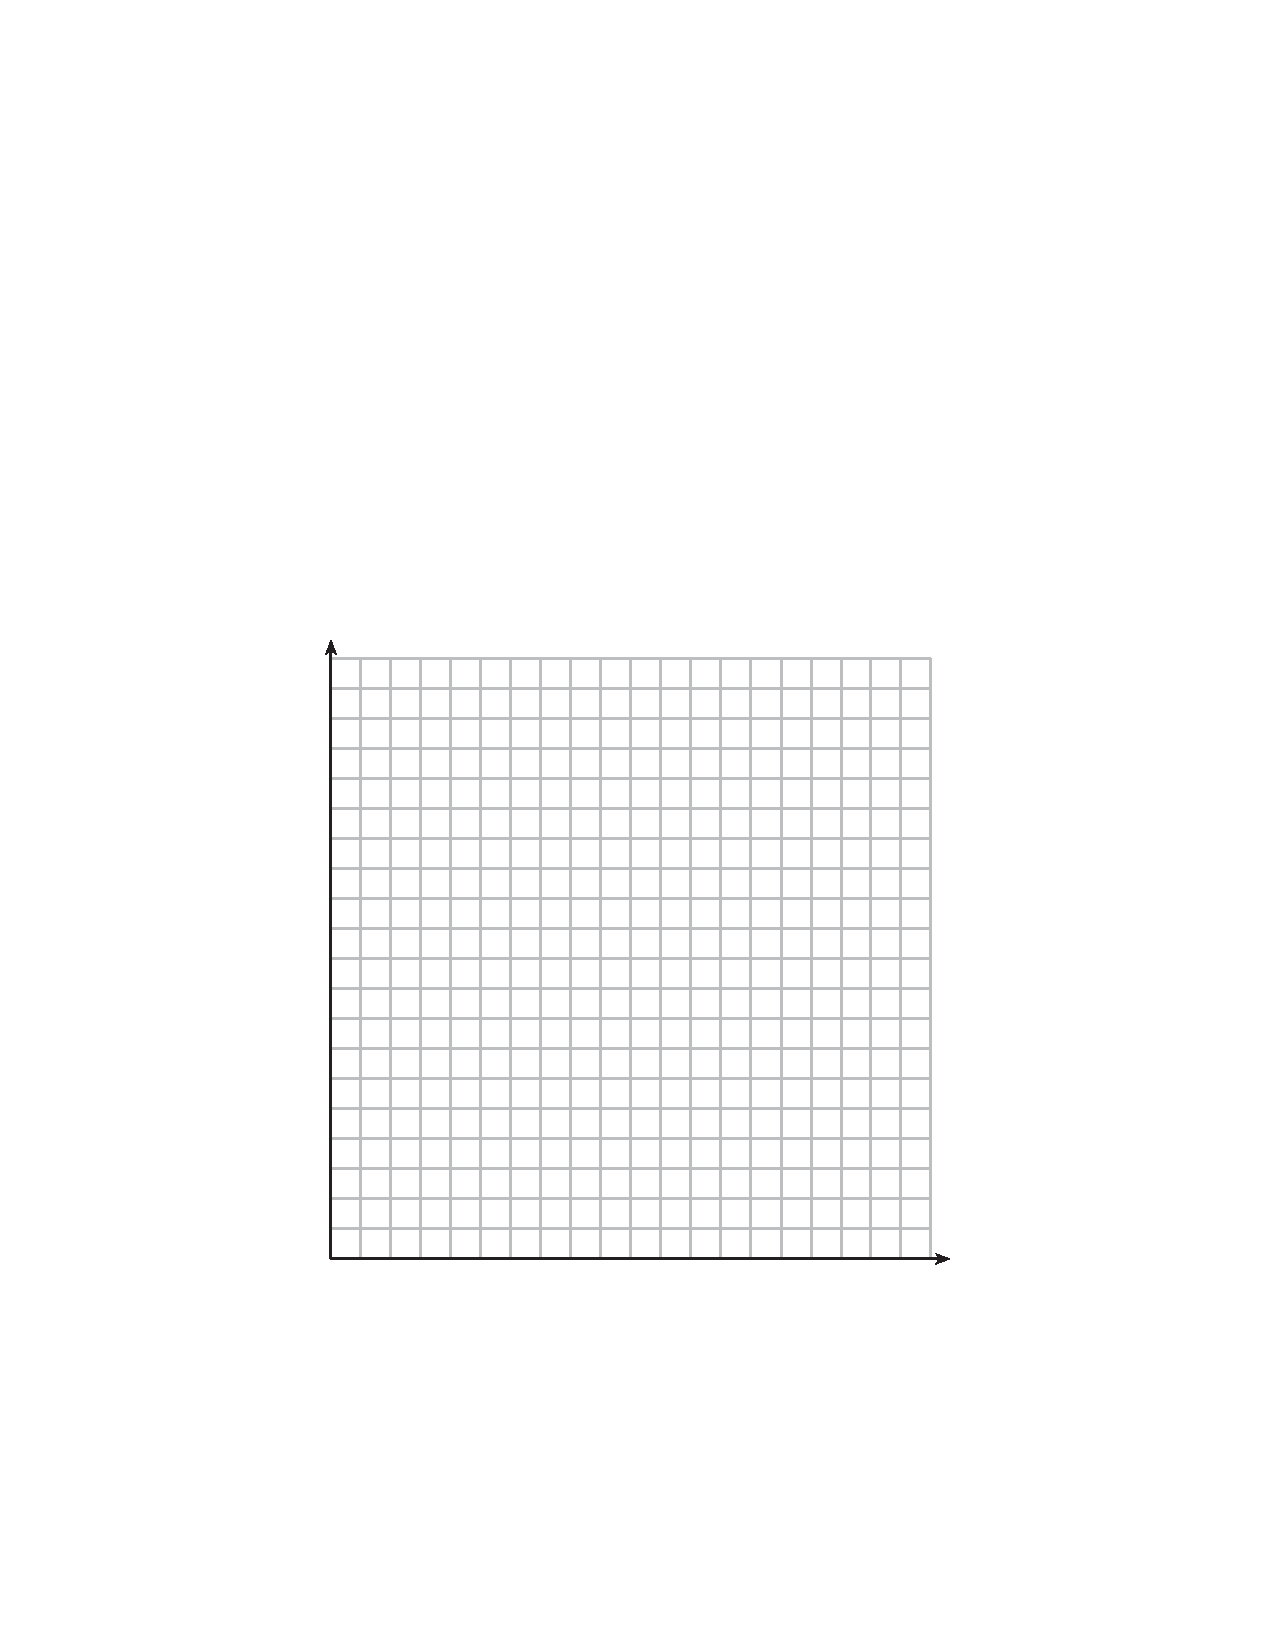
\includegraphics[width=0.85\textwidth]{1stQ-grid.pdf}
\end{figure}

\end{enumerate}
\end{document}